% Suppose the prefilling time of $x$ prompt tokens to be $P^M(x)$ for agent model and $P^m(x)$ for memory model and the decoding time of $y$ completion tokens to be $D^M(y)$ for agent model and $D^m(y)$ for memory model. For simplicity, assume the time to execute environment at each step is small enough to be negligible. We further suppose that $a$ and $o$ are always of the same size, so that we can omit the subscripts for now. In practice the environment execution time is hardly controllable and is a separate consideration from the system design. Thus, for the vanilla full-context version of agent, the latency at each step is $P^M(o) + D^M(a)$.

% In the basic {\model}, the compressed state and the policy are produced sequentially at each step, and thus the latency cost at each step is,
% \begin{equation}
%     P^M(s) + D^M(a) + P^m(a+o) + D^m(s)
% \end{equation}
% This is notably higher than before since the In $k$-\textit{step-off} ($k \geq 1$)  version of {\model}, the agent uses the previously compressed state to produce the policy and thus allows the compressed state and the policy to be produced at the same time. Thus at the summarizing steps, the latency costs are,
% \begin{equation}
%     \max(P^M(o_t) + D^M(a_t),  P^m(a_{t-1}+o_t)+D^m(s_t))
% \end{equation}
% Empirically, with a relatively small state size, we found that the left part is almost always dominating, and thus we can approximate it as $P^M(o_t) + D^M(a_t)$. In the next step, the agent has to prefill again with the new summarizations, thus the latency cost is,
% \begin{equation}
%     P^M(s_t + a_t + o_{t+1}) + D^M(a_{t+1})
% \end{equation}
% And then the steps thereafter will maintain the usual inference time as in full-context until the next summarization step. the average run time per step is,
% \begin{equation}
%     P^M(o_t) + D^M(a_t) + (P^M(s_t+a_t+o_{t+1}) - P^M(o_{t+1})) / k
% \end{equation}
% Therefore, this will actually produce higher latency which might be non-negligible when using smaller $k$. One approach to alleviate this is to prefill during the non-summarization steps simultaneously with the agent model decoding. Specifically, during the 
\begin{figure*}[t]
    \centering
    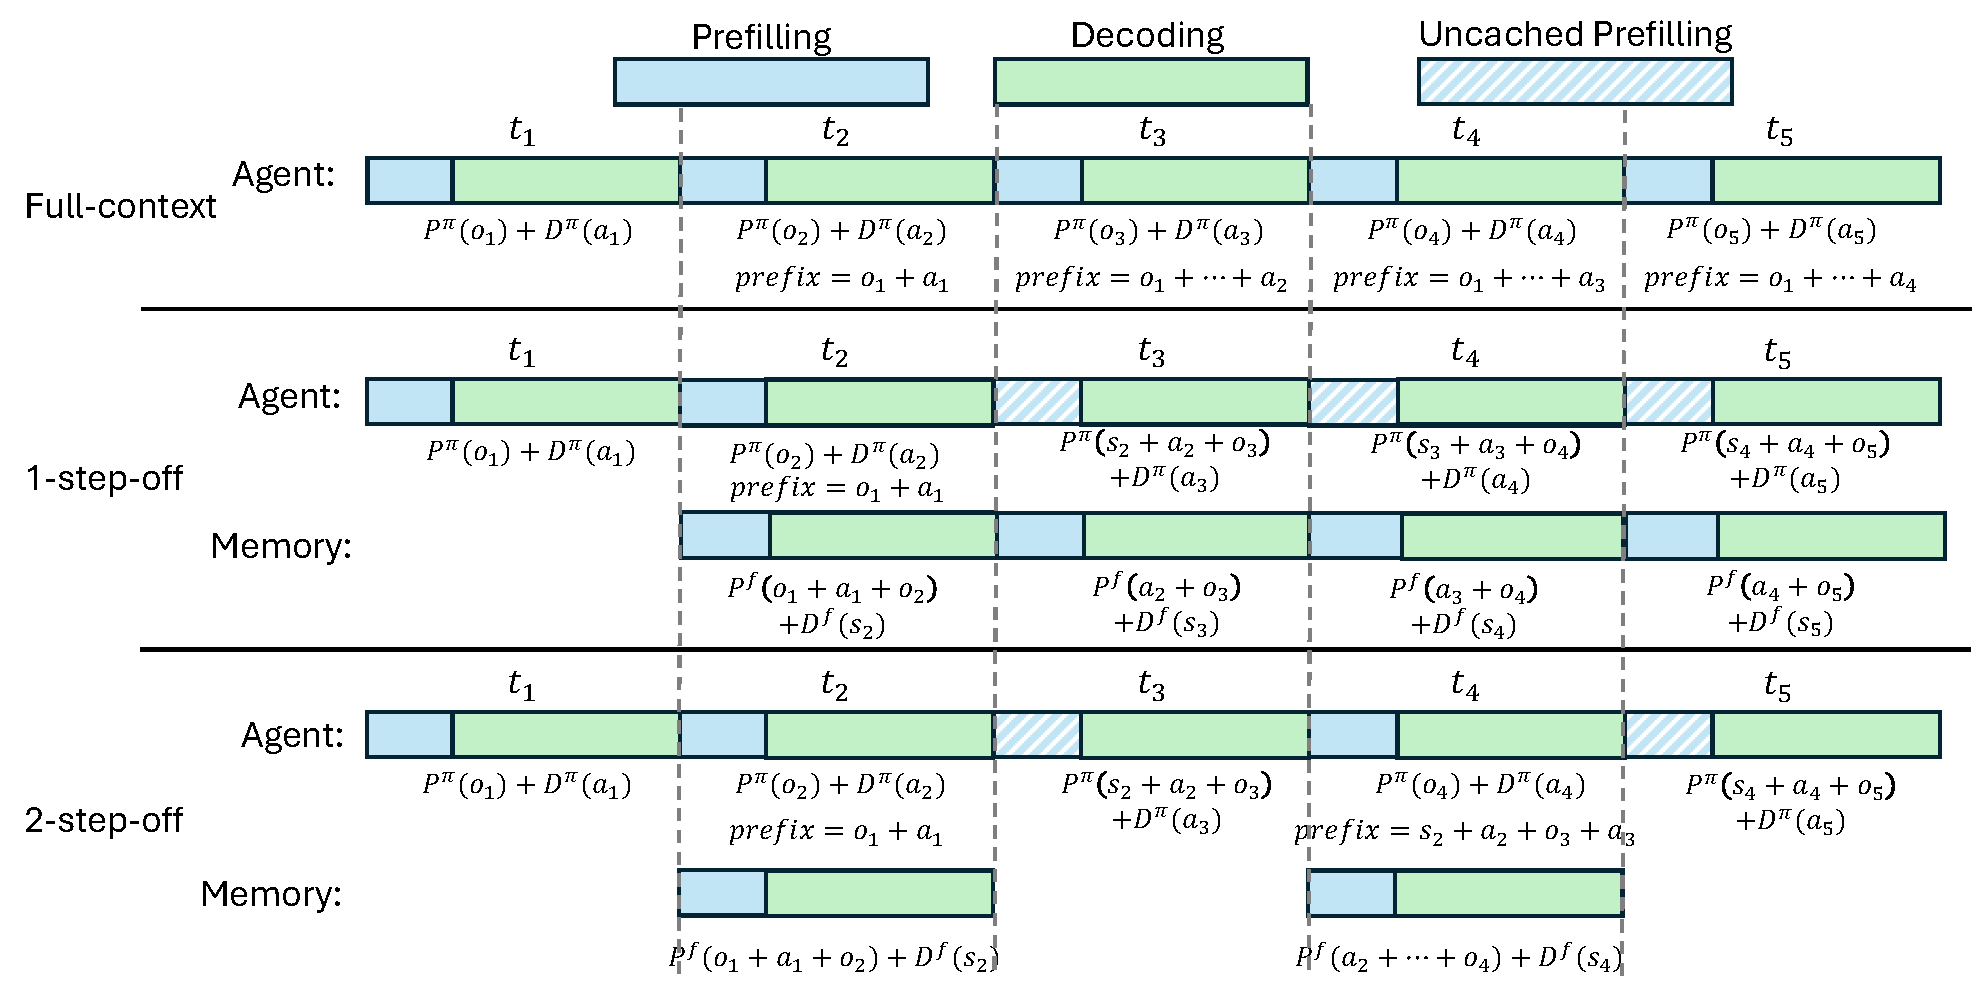
\includegraphics[width=0.94\linewidth]{figs/gantt4.pdf}
    \caption{Gantt chart illustrating the $k$-step-off pipeline. We denote $P^\pi(\cdot)$ and $D^\pi(\cdot)$ as the prefilling and decoding time of the agent model, and $P^f(\cdot)$ and $D^f(\cdot)$ for the memory model. Solid blue blocks denote cached prefilling (incremental), hatched blocks denote uncached prefilling (full context re-encoding after a summary update), and green blocks denote decoding. The ``prefix'' annotations indicate the cached KV prefix carried over from the previous step. When the prefix remains valid, only new tokens require prefilling. For $1$-step-off, every step after the first requires uncached prefilling due to the continuously updated summary. For $2$-step-off, the uncached prefill occurs only once per cycle, with the intermediate step reusing the cached KV prefix.}
    \label{fig:gantt}
    \vspace{-5mm}
\end{figure*}
% Suppose that the size of each KV is $S$ and the HBM bandwith is $W$. Then the saved time from {\model} compared with full-context counterpart is
% \begin{equation}
%     \Delta t = \frac{(L_{full}-L_{sum})S}{W}
% \end{equation}
% Suppose that the prefilling throughtput is $P$, then we will need to guarantee that the saved decoding time on $Y$ tokens can cancel out the summary prefilling latency.
% \begin{equation}
%     Y\frac{(L_{full}-L_{sum})S}{W} > \frac{L_{sum}}{P}
% \end{equation}
% Thus we can get
% \begin{equation}
%     \frac{L_{sum}}{L_{full}}<\frac{1}{1+W/YSP}
% \end{equation}
% Suppose serving a \texttt{Qwen/Qwen3-32B} on a single A100 GPU, where the HBM bandwidth is $W\sim 2\ \text{TB/s}$ and the prefilling throughput is $P=3,000 \ \text{tokens / s}$. And the KV size taken by each token is $2\times 10^{-4}GB$. Assume that the average number of completion tokens is $Y=1K$. Thus the ratio should be less than $0.43$.
While {\model} reduces memory overhead during the decoding stage, the introduction of the summary representation $s$ requires an additional prefilling stage for the agent model before further decoding, as shown in Figure~\ref{fig:gantt}.
To ensure a net reduction in end-to-end latency, the decoding speedup must sufficiently amortize the prefilling cost. We formalize this trade-off below.

\noindent \textbf{Theoretical Analysis}
Let $S$ denote the KV cache memory size required per token (in GB), and let $W$ represent the GPU's HBM bandwidth (in GB/s). Assuming the decoding process is memory-bound, the per-token latency reduction achieved by {\model} relative to the full-context baseline is:
\begin{equation}
\Delta t_{\text{decode}} = \frac{(L_{\text{full}} - L_{\text{sum}}) \cdot S}{W}
\end{equation}
where $L_{\text{full}}$ and $L_{\text{sum}}$ are the context lengths of the baseline and {\model}, respectively. However, generating the summary representation incurs a one-time prefilling latency. Assuming a prefilling throughput of $P$ (tokens/s), a net speedup requires that the cumulative decoding savings over $Y$ generated tokens exceed the prefilling overhead:
\begin{equation}
Y \cdot \underbrace{\frac{(L_{\text{full}} - L_{\text{sum}}) \cdot S}{W}}_{\text{Per-token decoding saving}} > \underbrace{\frac{L_{\text{sum}}}{P}}_{\text{Prefill cost}}
\end{equation}
Rearranging yields an upper bound on the permissible compression ratio:
\begin{equation}
\frac{L_{\text{sum}}}{L_{\text{full}}} < \frac{1}{1 + \frac{W}{Y \cdot S \cdot P}}
\end{equation}

\noindent \textbf{Case Study.} We instantiate this bound for \texttt{Qwen3-32B} served on a single A100-80GB GPU, with HBM bandwidth $W = 2$ TB/s, prefilling throughput $P = 3{,}000$ tokens/s, per-token KV size $S = 2 \times 10^{-4}$ GB, and average completion length $Y = 1{,}000$ tokens. Substituting these values yields $L_{\text{sum}} / L_{\text{full}} < 0.23$, which means for a prefix length of $32K$ tokens, we need to upperbound the summary length within $7.36K$ tokens. This is a compression ratio readily achievable through summarization.